\problemname{Vvvvvv}
Plattformspel är en gammal dataspelgenre där du rör dig på plattformar som hänger i luften. Vvvvvv är en sorts plattformspel där du inte kan hoppa, men istället kan växla mellan vanlig gravitation, som gör att du faller nedåt, och antigravitation, som gör att du faller uppåt. Förutom gravitationsomkopplaren (G) så finns bara två knappar i spelet, gå till höger (H) och gå till vänster (V).

I den här uppgiften ska du hitta en sekvens av knapptryckningar som tar dig genom en labyrintliknande uppsättning av plattformar och väggar, från en startposition till en slutposition. För att få full poäng ska sekvensen dessutom vara så kort som möjligt.

\begin{figure}[ht!]
\centering
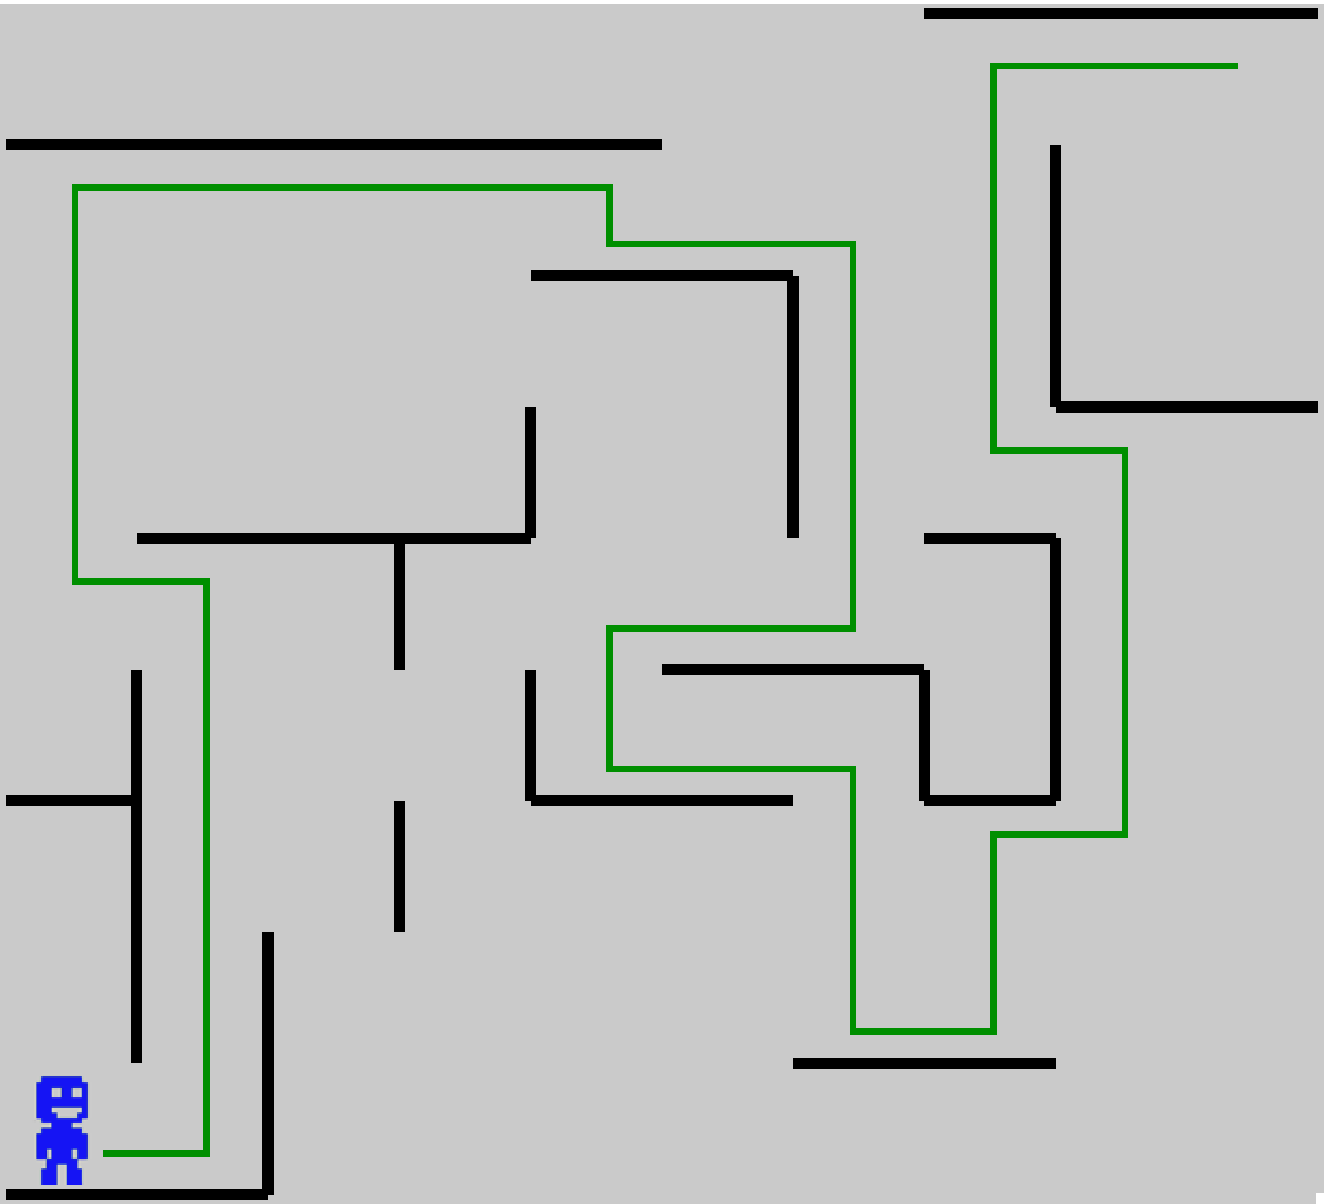
\includegraphics[width=0.6\textwidth]{spelplan.pdf}
\caption{Vägen som ges av knapptryckningssekvensen i det tredje exemplet.}
\label{overflow}
\end{figure}


\section*{Input}
Den första raden i indatan innehåller tre heltal $W$, $H$, och $N$: spelplanens bredd, spelplanens höjd samt antalet linjesegment. Därefter följer $N$ rader med fyra heltal $x_1$, $y_1$, $x_2$, $y_2$ på varje rad, där $0 \le x_1,x_2 \le W$ och $0 \le y_1,y_2 \le H$. Varje rad beskriver ett linjesegment med ändpunkterna ($x_1, y_1$) samt ($x_2, y_2$). Varje linjesegment är antingen vågrätt eller lodrätt, d.v.s. antingen gäller $y_1=y_2$ eller $x_1=x_2$. Heltalskoordinaterna kan sägas dela in den rektangulära spelplanen i ett rutnät, i vilket knappen V förflyttar dig en ruta åt vänster medan H förflyttar dig en ruta åt höger. Om du inte står på en plattform efter förflyttningen så faller du (uppåt eller nedåt) till närmsta plattform, och det finns ingen möjlighet att röra dig i sidled under fallets gång. Om du faller eller går ut ur spelplanen förlorar du spelet. Detsamma gäller om du försöker gå genom en vägg.

Startpositionen är rutan i nedre vänstra hörnet närmast punkten $(0,0)$ med gravitationen riktad neråt. Slutpositionen är rutan i övre högra hörnet, närmast punkten $(W,H)$. Det kommer alltid finnas ett linjesegment under startpositionen samt över slutpositionen.


\section*{Output}
Om det finns en lösning ska programmet skriva ut en sträng innehållande en bokstav för varje knapptryckning, valda bland H, V och G. Sekvensen ska ta dig från startpositionen till slutpositionen och måste vara kortare än $10\,000$ tecken. Du kan anlända till slutpositionen med valfri riktning på gravitationen, men du måste stå stilla, alltså ha "fallit färdigt" (se tredje exemplet nedan).

Om det inte finns en lösning ska programmet skriva ut strängen \texttt{"Inte"} (utan citationstecken).

\section*{Poängsättning}
Din lösning kommer att testas på en mängd testfallsgrupper. För att få poäng för en grupp så måste du klara alla testfall i gruppen.

\begin{tabular}{| l | l | p{5cm} | p{5cm} |}
	\hline
	Grupp & Poängvärde & Begränsningar & Krav \\ \hline
  1     & 20  & $W,H \le 10$, $N \le 25$, lösning finns med högst 10 drag & sekvensen behöver inte vara kortast möjlig. \\ \hline
  2     & 15  & $W,H \le 20$, $N \le 200$, lösning finns där man inte behöver använda V & sekvensen behöver inte vara kortast möjlig. \\ \hline
  3     & 15  & $W,H \le 50$, $N \le 2000$ & sekvensen behöver inte vara kortast möjlig. \\ \hline
  4     & 20  & $W,H \le 10$, $N \le 50$ & sekvensen ska vara kortast möjlig. \\ \hline
  5     & 30  & $W,H \le 100$, $N \le 5000$ & sekvensen ska vara kortast möjlig. \\ \hline
\end{tabular}
